\documentclass[tikz,border=2pt]{standalone}
\usepackage{tikz}
\begin{document}
  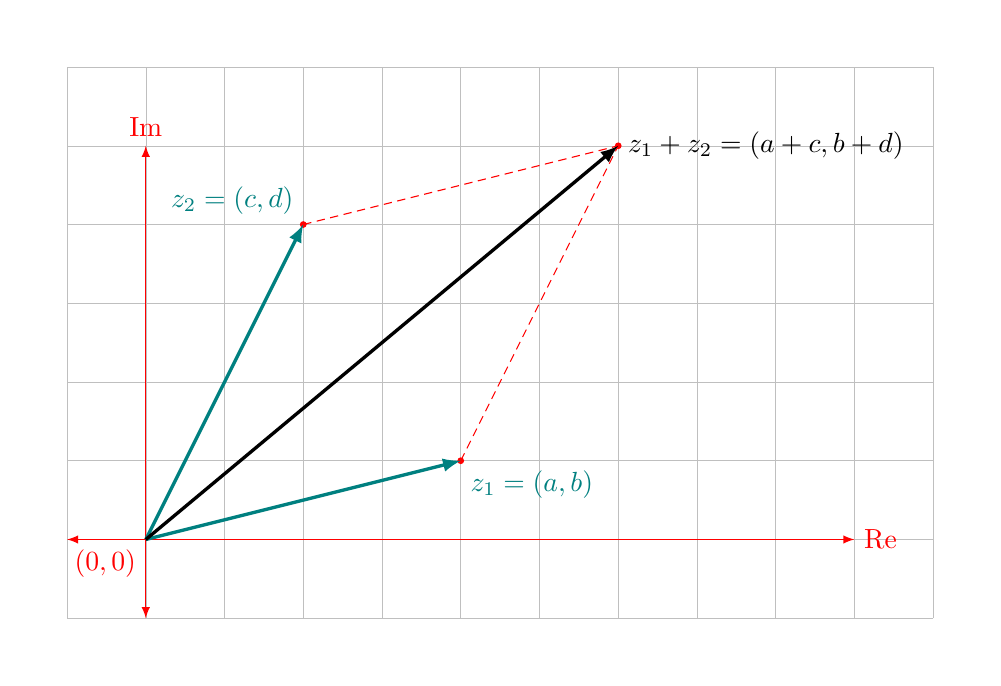
\begin{tikzpicture}
    \fill[white] (-1.5,-1.5) rectangle (10.5,6.5);
    \draw[lightgray,very thin] (-1,-1) grid (10,6);
    \draw (0,0) node[red,below left]{$(0,0)$};
    \draw[red,latex-latex] (-1,0) -- (9,0) node[right]{Re};
    \draw[red,latex-latex] (0,-1) -- (0,5) node[above]{Im};
    \draw[red,densely dashed] (4,1) -- (6,5);
    \draw[red,densely dashed] (2,4) -- (6,5);
    \filldraw[red] (6,5) circle(1pt) node[black,right]{$z_1+z_2=(a+c,b+d)$};
    \draw (4,1) node[teal,below right]{$z_1=(a,b)$};
    \filldraw[red] (4,1) circle(1pt);
    \draw[teal,very thick,-latex] (0,0) -- (4,1);
    \draw (2,4) node[teal,above left]{$z_2=(c,d)$};
    \filldraw[red] (2,4) circle(1pt);
    \draw[teal,very thick, -latex] (0,0) -- (2,4);
    \draw[very thick,-latex] (0,0) -- (6,5);
  \end{tikzpicture}
\end{document}

